\documentclass[11pt]{article}
\usepackage{geometry}                
\geometry{letterpaper}                   

\usepackage{graphicx}
\usepackage{amssymb}
\usepackage{epstopdf}
\usepackage{subfig}
\usepackage{amssymb, amsmath}
\usepackage{hyperref}
\usepackage{pdfpages}
\usepackage[framed,numbered,autolinebreaks,useliterate]{mcode/mcode}

\hypersetup{
    colorlinks,%
    citecolor=black,%
    filecolor=black,%
    linkcolor=black,%
    urlcolor=black
}

\usepackage{booktabs}
\DeclareGraphicsRule{.tif}{png}{.png}{`convert #1 `dirname #1`/`basename #1 .tif`.png}

\title{Desert Ant Behaviour: Modelling desert ants with a focus on movement and navigation}
\author{Georg Wiedebach, Wolf Vollprecht}
\date{\today} 

\begin{document}



\thispagestyle{empty}

\begin{center}
\includegraphics[width=5cm]{images/ETHlogo.eps}

\bigskip


\bigskip


\bigskip


\LARGE{ 	Lecture with Computer Exercises:\\ }
\LARGE{ Modelling and Simulating Social Systems with MATLAB\\}

\bigskip

\bigskip

\small{Project Report}\\

\bigskip

\bigskip

\bigskip

\bigskip


\begin{tabular}{|c|}
\hline
\\
\textbf{\LARGE{Insert Title Here}}\\
\textbf{\LARGE{...}}\\
\\
\hline
\end{tabular}
\bigskip

\bigskip

\bigskip

\LARGE{Name 1 \& Name 2}



\bigskip

\bigskip

\bigskip

\bigskip

\bigskip

\bigskip

\bigskip

\bigskip

Zurich\\
May 2008\\

\end{center}



\newpage

%%%%%%%%%%%%%%%%%%%%%%%%%%%%%%%%%%%%%%%%%%%%%%%%%

\newpage
\section*{Agreement for free-download}
\bigskip


\bigskip


\large We hereby agree to make our source code for this project freely available for download from the web pages of the SOMS chair. Furthermore, we assure that all source code is written by ourselves and is not violating any copyright restrictions.

\begin{center}

\bigskip


\bigskip


\begin{tabular}{@{}p{3.3cm}@{}p{6cm}@{}@{}p{6cm}@{}}
\begin{minipage}{3cm}

\end{minipage}
&
\begin{minipage}{6cm}
 \large Georg Wiedebach\\
 \href{mailto:georgwi@student.ethz.ch}{georgwi@student.ethz.ch}
\end{minipage}
&
\begin{minipage}{6cm}

\large Wolf Vollprecht\\
\href{mailto:wolfv@student.ethz.ch}{wolfv@student.ethz.ch}

\end{minipage}
\end{tabular}


\end{center}
\newpage

%%%%%%%%%%%%%%%%%%%%%%%%%%%%%%%%%%%%%%%


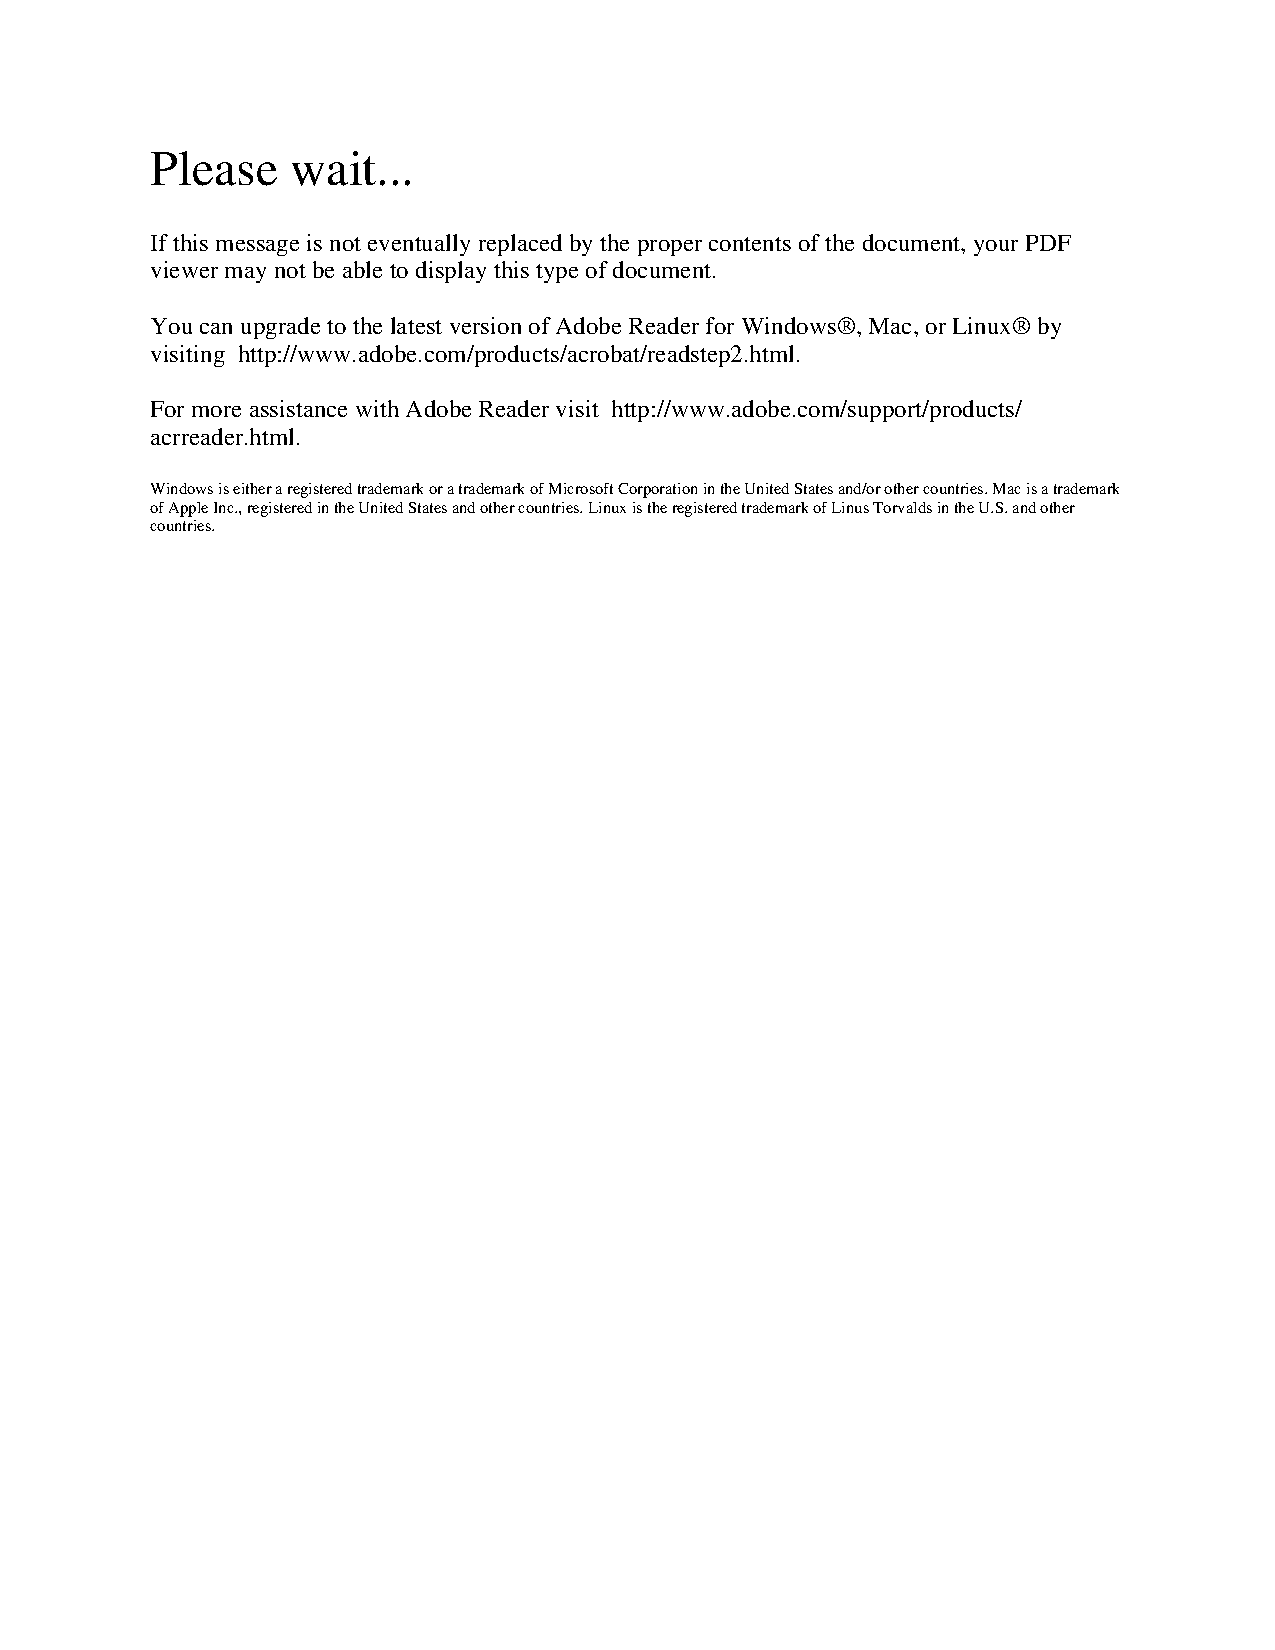
\includepdf{images/confirmation_en.pdf}
% IMPORTANT
% you MUST include the ETH declaration of originality here; it is available for download on the course website or at http://www.ethz.ch/faculty/exams/plagiarism/index_EN; it can be printed as pdf and should be filled out in handwriting

\begin{abstract}
This paper is the final result of the course {\sc Modeling Social Systems with MATLAB} which aimed to offer an insight into the MATLAB programming language and to use said language to model social systems with various different approaches. The timeframe of the course is one semester. \\
In this paper we will try to show how to replicate the behaviour of desert ants in a MATLAB simulation. Furthermore we will discuss our results and compare them to experimental results obtained by biologists.
\end{abstract}

\newpage

%%%%%%%%%% Table of content %%%%%%%%%%%%%%%%%

\tableofcontents

\newpage

%%%%%%%%%%%%%%%%%%%%%%%%%%%%%%%%%%%%%%%





\section{Individual contributions}
The whole project was done in a cooperative manner.
\newpage

\section{Introduction and Motivations}

We think ants are exciting animals because – despite their small body mass and therefore small brain – they form very huge and complex social structures. Very large numbers of them work together efficiently like one body. This requires a high level of coordination. We have already seen some videos which show the great achievements of ant colonies in building and hunting. Now we found out about their navigation abilities and are curious to learn how ants are able to cover extreme distances. The human being would definitely get lost when trying to journey this far in the desert without GPS or any other form of modern help, so one of our main goals will be to find out how ants can master this difficult task.

Ants have been subject of modern research since 1848, the motivations were often interest in their instincts, society and of course the hope to learn from them. Studies in ant movement became even more compelling when scientists started to look for algorithms that solve such fundamental tasks like finding the shortest way in a graph (Graph Theory). The class of ant colony optimization algorithms was introduced 1992 and has since been a field of active study.

However, those algorithms are using the behaviour of forest ants of the western hemisphere, which is not similar to the behaviour of desert in terms of choosing a good path and finding food. Since we are studying desert ants we had to take a different approach. Desert ants rely much more heavily on the few landmarks they find in their environment and less on pheromone tracks other ants have laid out before them, like forest ants do. Also they make use of a path-integrator with which they are able to track their position in reference to where they started the journey, most likely the nest.\\\\
Results of interest are:
\begin{itemize}
\item How optimized is navigation by vectors 
\item What is the most energy-consuming task
\item Out of which states is it possible for the ant to find the nest (e.g. dropping the ant somewhere else, outside of her regular path etc.)
\item How well does the ant learn in the course of repeated journey towards the food and back
\end{itemize}

Of course we were as well motivated to improve our knowledge of MATLAB\texttrademark

\newpage

\section{Description of the Model}
We would like to create a model of desert ant behaviour. This will include their search for food, their returning to the nest and their orientation with global and local vectors. Also we will see how close our algorithms are to real ant movement. Therefore we want to simulate the experiments described in the papers. Our model should be able to deal with different numbers of landmarks, obstacles and starting points. We would like to give our ants the ability to learn and improve their efficiency when searching and finding food.

Because of the nature of our problem we choose to design our simulation around a time-discrete step-based model of an ant. We chose to let only one ant run at a time, because we don’t think that an higher number of ants would make much of a difference considering the vast space in the deserts. Therefore we can leave out influences of near ants like separation and cohesion (compare Agent Based Modeling).

The simulation should be capable of finding a good path between nest and feeder and use a simple learning process to achieve that. We want to create a model, that can autonomous avoid obstacles and not get stuck in a corner. In order to meet this requirements we split our simulation in two parts:

\subsubsection*{Landscape}
Our landscape should contain all the information about
\begin{itemize}

\item Position of the nest
\item Position of the feeder
\item Obstacles (stones, trees, cacti, oases, sand dunes and many more), from which some can be used as landmarks
\end{itemize}

We chose to limit our landscape: We implemented fixed boundaries, which hinder the ant from escaping out of our experiment area. This is important to limit the time the ant needs to find food and thus making our simulation very less time-consuming. A matrix stores information about taken and free points by the values true or false, where false stand for an obstacle. Nest, feeder, landmarks and local vectors are saved separately as vectors, to make them easy to reach.
\begin{figure}[h!]
	\centering
 	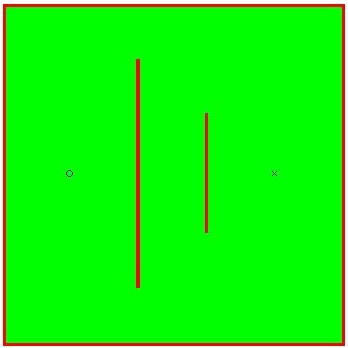
\includegraphics[scale=0.6]{images/landscape.jpg}
 	\caption{Example of a simple landscape: obstacles red, feeder and nest are indicated with x and o}
\end{figure}
\subsubsection*{Ant}
Our ant should follow certain, simple rules to move according to the studies we received as part of the project description. Such are basic rules like avoiding obstacles or a little more specific rules like following the global vector when returning to the nest and using the local vectors of the landmarks when finding the food again. During the simulation and after the ant has had success in finding food our local vectors should as well change according to the new found and better path.

\subsection{Simplifications}
There will be simplifications and assumptions, the most important ones are:
\begin{itemize}
\item We decided to create fixed boundaries on our Landscape.
\item For our model we strictly separate navigation by global vector (feeder to nest) and by local vectors (nest to feeder). This is due to the fact that this behaviour can differ from ant to ant and there is no consistent result true for all desert ants.
\item The model will have a “detection-radius” in which landmarks, nest and feeder are considered for moving and navigating.
\end{itemize}
\newpage

\section{Implementation}
As described above our simulation consists of two main parts: The landscape and the ant. Both of these were implemented as separate classes. A third class the simulation-class should handle the rendering, initialising and iterations. We also used a main-file in which we declared variables that would have impact on the outcome of our simulation like the detection-radius of the ant or information on the map, that should be loaded.
\subsection{Landscape}
The landscape class only contains information about the map, the nest and the feeder as well as some spots which are landmarks, used by the ant as anchor points for local vectors.

We implemented different versions of loading landscapes into our simulation. Beside the possibility of creating the landscape-matrix in a separate m-file and the random-map generator  we often used a simple but elegant method for generating maps out of arbitrary made generic Portable Network Graphics. This method finds specific color values and translates them into their meaning in the context of the landscape.

\begin{table}[h!]
\centering
\begin{tabular}{lll}
	\cmidrule[1pt]{2-3}
	& Color in png-file & Color in Matlab \\
	\midrule
Obstacle & black & red \\ \midrule
Nest & green & black circle \\ \midrule
Feeder & blue & black cross \\ \midrule
Landmark & turquoise & blue circle \\
\bottomrule  
\end{tabular}
\caption{Color values and their meaning}
\end{table}

\begin{figure}[h!]
	\centering
	\subfloat[Original image]{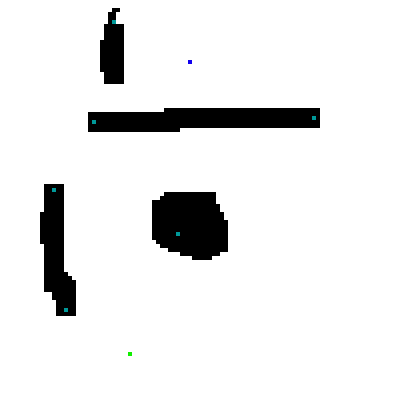
\includegraphics[scale=0.4]{images/map2skal.png}}
	\subfloat[Generated landscape]{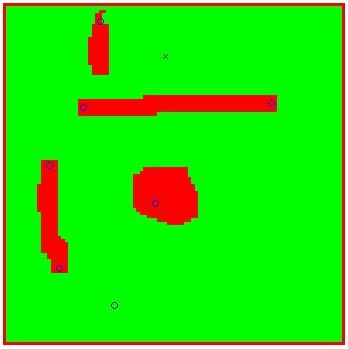
\includegraphics[scale=0.5]{images/map2.jpg}}
	\caption[Generating a map from image]{Generated map from image}
\end{figure}

\subsection{Ant}

The class \texttt{ant} mainly contains the current position of the ant, the local vectors on landmarks and the path integrated global vector which should always point to the nest (as long as the ant moves are coherent).
We built our ant around the most important method: \texttt{move}. The  \texttt{move} function is called out of two different methods the  \texttt{find\_food} and the \texttt{return\_to\_nest}. In the following all methods of the class \texttt{ant} are described:

\subsubsection{Find food} This loop iterates the move-method until the ant reaches the food. Depending on how often the ant has already been on the track, it uses the aggregated local vectors to calculate a direction which the ant should follow to reach the food sooner. As soon as the feeder is in a certain distance (the detection radius) the ant runs straight towards it.

\subsubsection{Calculate the direction from landmarks}
\begin{equation}
	\vec{v}_{direction} = \sum_{i=0}^{n}\vec{l_i} \quad \forall ||\vec{l_i}||_2 < r_{detection}
\end{equation}
where $\vec{l_i}$ are the local vectors, $i$ ranging from the first to the last landmark and $r_{detection}$ is the view radius of the ant.

\subsubsection{Return to nest}
When returning to the nest, the model uses the same move method as when 	searching, but instead of calculating a general direction out of the occurring local vectors the ant uses the global vector, which always leads straight back to the nest. While returning to the nest it updates all local vectors while passing the related landmarks. In our implementation the local vectors always points to the last landmark the ant has passed or are adjusted toward this position. Thereby the ant develops a steady route that is a close to the optimal route. Of course there is no possibility to find out how real ants remember the exact direction and length of the local vectors and therefore this way of implementation must be tested for reliability later on.

\subsubsection{Updating the local vectors on all landmarks}

For the implementation we decided, that our model of the ant, would be able to remember only the last global vector where a landmark was spotted. This simplification seems to be adequate because of the limited brain complexity of real ants. For this reason the model, when spotting a new landmark always calculates a vector pointing to the latest landmark and thus developing a path that leads from the first landmark, the nest, to the latest, which should be quite close to the feeder. This implementation however will result in non-changing local vectors after the first run. So we included a \textit{grow-factor}, which only allows a small adjusting every time the ant passes the landmark. As a result the learning curve of the ant became interesting, as described below in the experimental results.

\begin{eqnarray}
a & = & 0.5 * \exp \left(-\frac{||\vec{l_i}||_2}{10}\right) \\
\vec{l_i} & = & a * \text{round} \left(\vec{l_i}  + \left(\vec{g_i} - {\vec{g}_{i-1}}\right)\right)
\end{eqnarray}

\subsubsection{Move} 
The move method is heart of the ant class: it accepts any general direction vector as input and sets the new position of the ant as a result. A general direction input can be calculated in the method “find food” or “return to nest”. It also handles all the checking for obstacles. Move is invoked in every time-step. Because the ant has only a choice of 8 possible next positions the method must calculate a new direction vector to one of the first order Moore neighbours:


To calculate the matching Moore neighbour from the general direction vector we use the following formula and call the result the “main-direction”.

\begin{equation}
\vec{m} = \text{round}\left(\vec{dir}*\frac{1}{\text{max}|dir_i|}\right)
\end{equation}

In case the general direction is not exactly a multiple of a vector given by the Moore neighbourhood this calculation will result in a non-natural path (s. picture below). So we calculated a “second-direction” which is chosen as move direction with a certain probability depending on the angle between the general direction and the main direction. This allowed to walk directly towards a target. Some limit cases are handled separate.

\begin{eqnarray}
\vec{s} & = & \vec{m}-\vec{dir} * \text{min} \left( |dir_i| \right) \\ 
p & = & \frac{\text{min}|dir_i|}{\text{max} |dir_i|}
\end{eqnarray}

If there is no general direction given to the method move, or if the general direction is zero a vector is generated based on the previous move direction. This vector then is turned around +/- 45 degree with a certain probability. This probability defines how twisted the ants path is. The following picture was taken with a low turning-probability (10 percent).

In the picture it is easily seen, that the ant can not move trough obstacles. This is also part of the method move. Therefore the method checks the desired position on the map. If the position is not available the move-vector is turned around 45 degree clockwise or counter-clockwise, then the desired position is checked again until a possible step is found.

\begin{figure}[h!]
	\centering
	\subfloat[Without second direction]{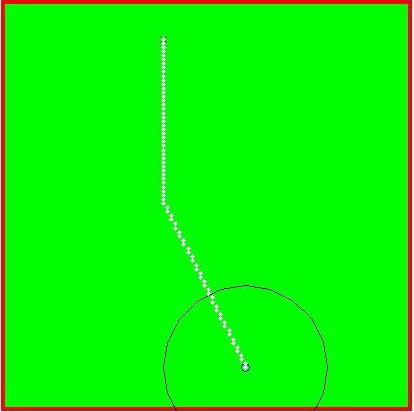
\includegraphics[scale=0.5]{images/mainvec.jpg}} \hspace*{1cm}
	\subfloat[With second direction]{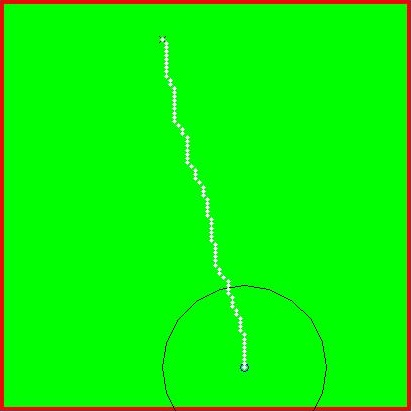
\includegraphics[scale=0.5]{images/secvec.jpg}}
	\caption[Comparison: Using second direction or not]{Calculating move direction with and without second direction}
\end{figure}
\begin{figure}[h!]
	\centering
	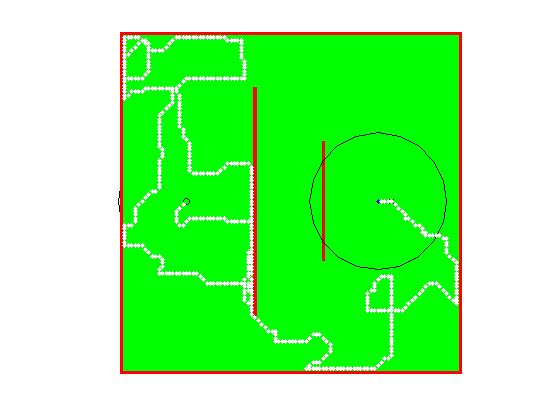
\includegraphics[scale=0.6]{images/foodsearch.jpg}
	\caption[Ants first search for food]{First search for food. No local vectors are set.}
\end{figure}
\subsection{Simulation}
The simulation class main purpose is to serve as a holder for the landscape and the ant. It also handles everything that has to do with output. The most important functions are the run-method, and the render-method, these two are described below.
\subsubsection{Run}
In this method there are basically two while-loops checking whether the ant is searching for food or trying to return to the nest. This is indicated by two Boolean values in the class ant. In each cases the corresponding ant-methods are invoked. Here is a simple example of using parts of the run-method (pseudo code):
\begin{lstlisting}
while the ant has no food
	search for food and move one step
	if the simulation needs to be rendered
		render the actual position of the ant on the map
	end
end
\end{lstlisting}

\subsubsection{Render} 
We soon realised that rendering the output while simulating is the main bottleneck in terms of time consumption. That is why we made it optional, so that it can be turned on or off for every simulation instance in the main-file. Another speed-improvement made here is achieved by not plotting the whole map but only the and an the detection-radius. Local vectors are rendered in a different method after each successful returning to the nest.

\newpage
\section{Simulation Results and Discussion}
\subsection{Expected Results}
We expect our simulation to be able to find short paths from Point A to desired position B, in this case nest to feeder and feeder to nest. We will try to be as close to nature as possible and hope to be able to recreate some of the experimental results given. Some results we consider particularly interesting are avoiding obstacles on returning home and the use and improving of local vectors. Of course there sure are models of desert ant behaviour already, because these animals are topic of research for a long time, but our simulation is mostly based on our own consideration so we are especially tense whether our results are accurate.
\subsection{Experimental Results}
\subsubsection{Path Integration Experiment}
The first run of our simulations completely reproduced a real experiment, given in the paper by R. Wehner\cite{wehner03}. The main purpose is to learn how effective and realistic the implemented model behaviour is.

In the Experiment the ant is allowed to find food and then has to return to the nest with a correct global vector. To increase the difficulty two obstacles are placed between the nest and the feeder to study the return-behaviour of the ants. This interference is made after the ant reaches the nest without obstacles.

To reproduce this situation we set our “ant” at the feeder and adjusted the correct global vector to the nest. Our results are mostly the same as the results seen in the experiment. Only one thing differs in our model: The real ant always chooses the same direction to turn at the obstacle. This might be the result of a simple payoff-learning process, once effective there was no need for the real ant to change the way. Unfortunately the experiment is not repeated with a higher number of different ants.

\begin{figure}
	\centering
	\subfloat{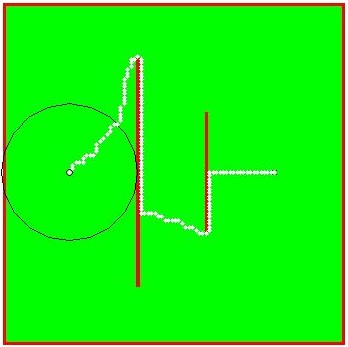
\includegraphics[scale=0.4]{images/return1.jpg}}
	\hspace{1cm}
	\subfloat{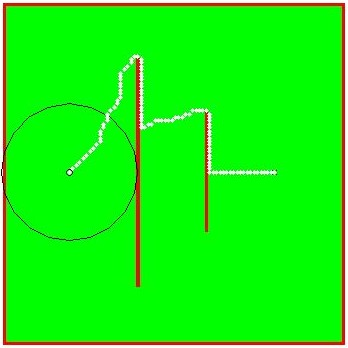
\includegraphics[scale=0.4]{images/return2.jpg}}
	\caption{Returning to nest with global vector}
\end{figure}

In the two pictures above two of our result-paths are shown. Obviously the simulated ant tries to go directly to the nest. Once there is a obstacle in the way the path turns randomly left or right until the obstacle is passed. Then the direct way to the nest is chosen again. During the time of wandering along the obstacle the global vector is adapted every step the ant takes.

In this specific case the model is reproducing the real experiment very accurate. There are still some questions open: whether the real ant at a obstacle indeed turns left or right based on a random decision is not clear. But as the experiment given only uses one single ant this question can not be answered.

\subsubsection{Food searching by local vectors}
In the implementation the local vectors are updated every time the ant reaches the nest. The following picture shows the path taken by the ant in her fourth run to the feeder. On each of the red obstacles there is a landmark with the associated local vector (yellow). If there is a landmark in the “detection-radius” of the ant, visualized by the black circle, the ant considers the local vector for the path. Of course the detection-radius is crucial in this experiment so we tried the same run with different values on a slightly different map.
\begin{figure}[h!]
	\centering
	\subfloat{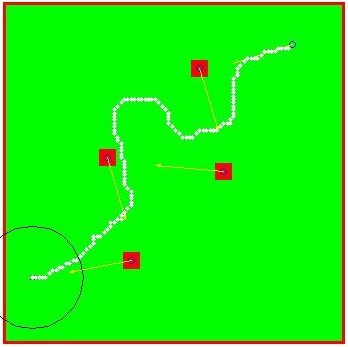
\includegraphics[scale=0.4]{images/view_small.jpg}}
	\hspace{1cm}
	\subfloat{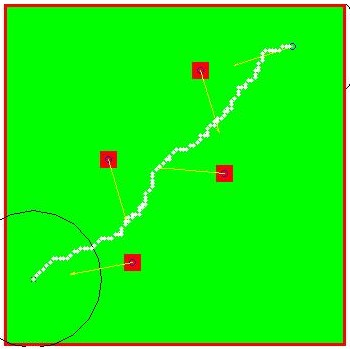
\includegraphics[scale=0.4]{images/view_medium.jpg}}
	\\
	\subfloat{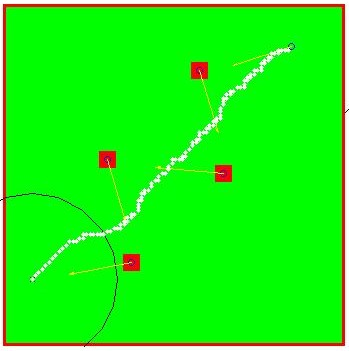
\includegraphics[scale=0.6]{images/view_large.jpg}}
	\caption[Comparing growing detection radius]{Comparison of different sizes of the detection radius}
\end{figure}
Above there are three runs of the same simulation with different detection-radius (black circle around the ant). Naturally the path becomes more direct the more landmarks the ant can see at one time step, because the local vectors are summed up. In the first picture the smallest view radius is simulated and in the beginning it is really easy to see, at which points the landmarks come in to view. Between the second and third mark the ant “looses” the path for a short time.

\subsubsection{Path Improvement}
In the following we tested several maps and landmark-arrangements and graphed the number of steps the ant needed to find food and returning to the nest. Of course once the local vectors were set and updated the step-number decreased. In the picture you can see the map we used for the results discussed below.
\begin{figure}
	\centering
	\subfloat[Map with local vectors]{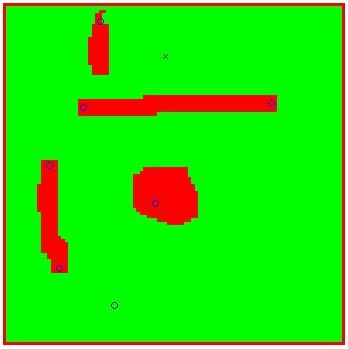
\includegraphics[scale=0.4]{images/map2_withlocal.jpg}}
	\subfloat[]{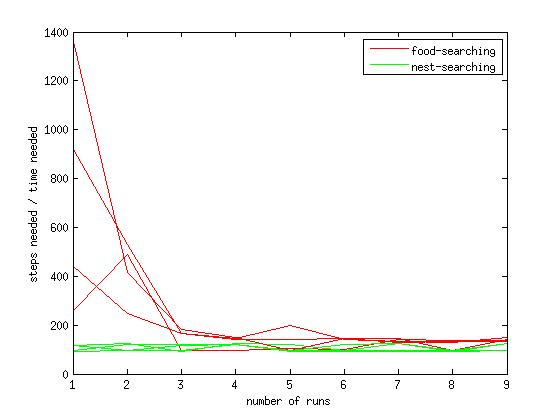
\includegraphics[scale=0.35]{images/pi.jpg}}
\end{figure}
A improvement can be seen clearly until the fourth or fifth time the ant has to reach the feeder. Until then the local vectors are not improved anymore [Footnote Video]. Another interesting fact seen in this graph is, that the navigation by local vectors never reaches the same level of effectiveness as navigating back to the nest by the global vector. The results can differ in other maps with more or less landmarks, but some aspects are always the same:
\begin{itemize}
\item Global vector navigation is in most cases more efficient than local vector navigation.
\item In the first few runs the fall of needed steps is highest.
\item On some map arrangements it is not possible for our model to improve. This happens if there are to few local vectors or the detection-radius is to small.
\end{itemize}

\newpage
\section{Summary and Outlook}
\subsection{Results}
In this paper we showed that the model was able to replicate the path pattern of ants, when searching randomly for food, when returning to the nest by global vector and when using local vectors to search for food through a simple agent-based model. Most of the experiments described by Wehner[footnote] were recreated and our modeled ants behaved indeed similar to the given results.
\subsection{Further Improvments}
One of the most obvious improvements to our model must be the inclusion of local vectors when returning home. Ants navigate with a certain chance by landmarks instead of the global vector on their way back to the nest as is showed in [[Wehner, 1998]]. This is a complication, but can clearly improve the steps needed when returning home. Especially with a defective or even wrong global vector this can be very helpful when searching for the nest. This situation was not part of our model experiments and is therefore listed in our simplifications.

Also, we noticed that our model sometimes got stuck on random generated maps, when caves, small holes and certain patterns occurred. Our artificial made experimental maps where free of those trouble generating conditions, so that our model still produces valid results, but the improvement of the move method in the class ant definitely should be considered when further improvements are done.

Another question of interest is, how our model would behave if we gave it a higher degree of freedom in terms of moving. For now we have limited the move radius to the first order Moore Neighbours. One could also think of a ant, that can watch several steps ahead in order to find out which positions are desirable, creating a better path and realising obstacles earlier.

While running, our model uses the local vectors only as long as they stay in the view radius of the ant, therefore forgetting about them as early as they went out of sight. The same holds true for the detection of the food. This leads in some situations to the loosing of track, even after the food was in the detection radius of the ant. A more realistic approach would be to make the model “slowly forget” about the landmark or the position of the feeder.

\newpage
\appendix

\section{Research Plan}
\textbf{Group Name:} The Anteaters Are Back\\ \\
\textbf{Group participants names:} Wolf Vollprecht, Georg Wiedebach

\subsection{General Introduction}

We think ants are exciting animals because – despite their small body mass and therefore small brain – they form very huge and complex social structures. Very large numbers of them work together efficently like one body. This requires a high level of coordination. We have already seen some videos which show the great achievngs of ant colonies in building and hunting. Now we found out about their naviagion abilities and are curious to learn how ants are able to cover extreme (in comparison to their own body size) distances. The human being would definitely get lost when trying to jurney this far in the desert wthout GPS or any other form of modern help, so one of our main goals will be to find out how ants can master this difficult task.

Ants have been subject of modern research since 1848, the motivations were often interest in their instincts, society and of couse the hope to learn from them. Studies in ant movement became even more compelling when scientists started to look for algorithms that solve such fundamental tasks like finding the shortest way in a graph (Graph Theorie). The class of ant colony optimization algorithms was introduced 1992 and has since been a field of active study.

\subsection{Fundamental Questions}
\begin{itemize}
\item How does ant movement and navigation work in challenging environments such as the desert?
\begin{itemize}
\item Is ant communication connected to ant navigation?
\item Which mechanisms and factors influence ant movement?
\item Are there different strategies to find the shortest/safest etc. path?
\end{itemize}
\item How can we describe ant paths in mathematical terms?
\begin{itemize}
\item How efficient are our mathematical models of the real ant behaviour?
\end{itemize}
\item How does our finding apply to the real world?
\end{itemize}
We would like to create a model of desert ant behaviour. This will include their search for food, their returning to the nest and their orientation with global and local vectors. Also we will see how close our algorithms are to real ant movement. Therefore we want to simulate the experiments described in the papers. Our model should be able to deal with different numbers of landmarks, obstacles and starting points. We would like to give our ants the ability to learn and improve their efficency when searching and finding food. Of course there will be some simplifications we eventually will have to deal with: Such as ... will be updated during work on the simulation.

\subsection{Expected Results}

We expect our simulation to be able to find short paths from Point A to desired positon B (i.e. feeder, nest) and back. We will try to be as cose to nature as possible and hope to be able to recreate some of the experimantal results given. Some results we consider particulary interesting are avoiding obstacles on returning home or finding a way to the nest after being deffered to a place where our ant has a non-fitting global vector. Of course we hope that there are already some good mathematical models available on ant movement, because these animals are topic of research for a long time already.

The evolution may have taught ants a lot of useful tricks and methods to survive in environmets like the desert. Probably there are more ways to orientate than only by landmarks. Ants may have similar ways to find out their geographic orientation like pigeons, or use the sun as a fix-point. We are curious to find out more about that.


\newpage
\section{MATLAB Code}
\subsection{main.m}
\lstinputlisting{../code/main.m}
\subsection{simulation.m}
\lstinputlisting{../code/simulation.m}
\subsection{landscape.m}
\lstinputlisting{../code/landscape.m}
\subsection{ant.m}
\lstinputlisting{../code/ant.m}

\newpage
\section{References}

\bibliographystyle{plain}
\bibliography{references}

\listoffigures




\end{document}  
